\documentclass[prl,showpacs, twocolumn]{revtex4-1}
\usepackage{graphicx,amssymb,color}
\usepackage[dvipsnames]{xcolor}
%\usepackage[utf8]{inputenc}
\usepackage[spanish]{babel}
\usepackage{pgfgantt}


\begin{document}
\title{FI3104 M\'etodos Num\'ericos para la Ciencia e Ingenier\'ia\\ Tarea 10}
\author{Camila Sandivari}
\affiliation{Profesor: Valentino Gonzalez \\ Profesor Auxiliar: Felipe Pesce}
\date{\today}

\begin{abstract}
En el presente reporte mostraremos el an\'alisis y ajuste de un espectro utilizando dos modelos distintos, uno utiliza la Gaussiana y el otro un perfil de Lorentz. La espectroscop\'ia estudia la interacci\'on de las ondas electromagn\'eticas con la materia como absorci\'on o emisi\'on de energ\'ia radiante, en este caso, vemos una linea de absorci\'on e intentamos simularla lo mejor posible, para esto optimizamos la funci\'on que define la diferencia entre los modelos y los datos. Podemos aprender tambi\'en el m\'etodo de test de Kolmogorov-Smirnov para evaluar cual de los m\'etodos se ajusta mejor a los datos.
\end{abstract}
\maketitle

\paragraph{Procedimiento}
\subparagraph{Parte 1}

Se utiliza como modelo una linea recta (1) y se le sustrae una Gaussiana (2) en el caso (a) y un perfil de Lorentz (3) en el caso (b). Para implementar las funciones se utiliza el paquete $scipy.stats$, en el caso de la Gaussiana es $scipy.stats.norm$ y el Perfil de Lorentz es $scipy.stats.cauchy$. Ambas reciben como par\'ametros la amplitud $A$, la varianza $\sigma$ y el centro $\mu$.  Entonces se tienen cinco par\'ametros para cada modelo, los tres par\'ametros de las funciones (Gaussiana, Perfil de Lorentz) y los dos par\'ametros de la l\'inea recta $a$ y $b$. Una vez establecido el modelo, se minimiza la funci\'on de $\chi^2$ correspondiente mediante la funci\'on $Leastsq$ del paquete optimize (Como se explic\'o en el reporte anterior esta funci\'on minimiza $\chi^2$ usando el m\'etodo levenberg-marquardt), esto nos entrega los cinco par\'ametros que optimizan cada ajuste.

Volviendo a los modelos, con los par\'ametros adecuados, se grafica ambos sobre los datos y observar el ajuste.

\begin{center}
\begin{eqnarray}
y= a x +b\\
f(x) = a\exp (-(x-b)^{2}/2c^{2}) \\
f(x)= \frac{1}{\pi(x^{2}+1)}
\end{eqnarray}
\end{center}

\subparagraph{Parte 2}
Para evaluar si los m\'etodos son buenos o no, m\'as a\'un, para evaluar cual de los dos es "mejor" se utiliza un test de Kolmogorov-Smirnov, que esta implementado en el paquete $scipy.stats$ como $kstest$.

\bigskip
\paragraph{Resultados}
\subparagraph{Parte 1}
Cuando se minimiza $\chi^2$ se obtienen los par\'ametros para ambos m\'etodos, se pueden observar en el cuadro 1, incluyendo la correspondiente minimizaci\'on. Con estos par\'ametros se encuentran los ajustes, la figura 1 muestra ambos ajustes para los datos que se est\'an utilizando.

\begin{table*} [h!]
\centering
\begin{tabular}{|p{3cm}|p{2cm}|p{2cm}|p{2cm}|p{2cm}|p{2cm}|p{2cm}|}
\hline
M\'etodo & $A$ & $\mu$ & $\sigma$ &a&b& $\chi^2$ \\
\hline
 Gaussiana&  8.22 e-17 & 6.56 e+03 & 3.26 e+00 &  8.88 e-17  & 8.88 e-17& 5.20 e-35\\\hline
 Perfil de Lorentz&  1.11 e-16 & 6.56 e+03 &3.22 e+0& 7.92 e-21 & 8.81 e-17 & 5.00 e-35\\
\hline
\end{tabular}
\caption{Par\'ametros obtenidos en la minimizaci\'on de $\chi^2$ para c\'ada m\'etodo }
\label{ }
\end{table*}



\begin{figure} [h!]
\begin{center}
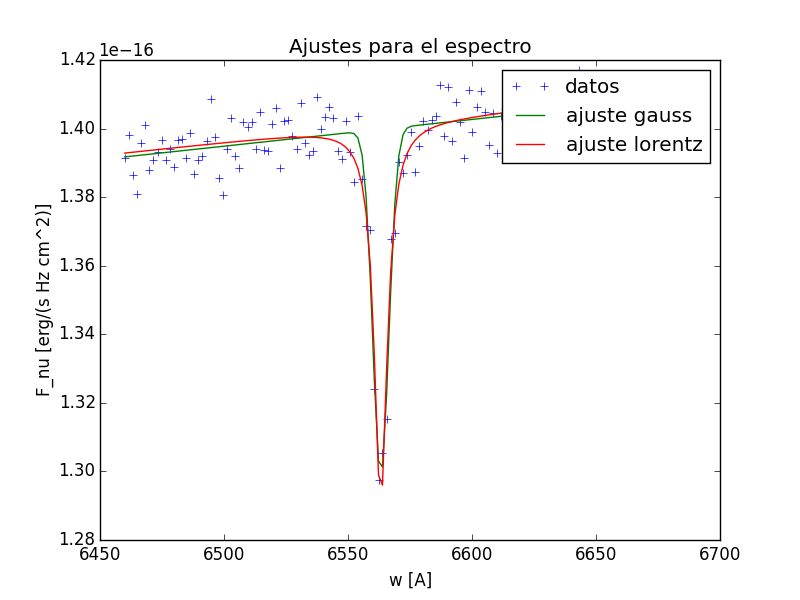
\includegraphics[width=4in]{1.png}
\caption{Gr\'afico con los ajustes de cada m\'etodo sobre los datos obtenidos para el espectro}
\label{ }
\end{center}
\end{figure}

\newpage
\paragraph{Conclusiones}
Tanto el perfil de lorentz, osea la distribuci\'on de cauchy, como la Gaussiana pueden ser utilizadas para generar un modelo que se ajuste a una linea de absorci\'on de un espectro. Este ajuste se optimiza mediante la funci\'on $\chi^2$ encontrando en este caso los 5 par\'ametros. 

\end{document}